\setcounter{chapter}{1} 

\chapter{Lightning}

\section{Natural Lightning}
The study and observations of lightning has a very long history, but only in the last century have we acquired the means to thoroughly investigate the electrical and meteorological mechanisms resulting in a thunderstorm.

There are varying theories in  the still open field of thunderstorms. The electrification mechanisms and the general electrical structure of the convective thunderstorms. This is further complicated by the fact that there seems to be different mechanisms at work for different scales of convective systems. Alas, every thunderstorm is a cloud, so it is necessary to explain cloud creation mechanisms.

The \textit{typical} lightning storm is created in summertime, this is caused by incoming solar radiation heating up the ground, and creating an unstable atmosphere.

The instability can be understood by recognizing that warm air is lighter than cold air, and therefore will rise. When air rises, less pressure is exerted on it, since the atmosphere is densest at the surface. This lower pressure causes work to be done by the rising air, to expand to a new equilibrium. The work done by the air in form of expansion, leads to a cooling of the air mass.

This instability is cause to a vertical movement. This vertical movement carries with it humid air. When the air mass is cooled by the expansion, the ability to hold water vapor is decreased (CC), and this may lead to condensation of vapor into liquid water in form of cloud droplets. Condensation of water vapor heats the surrounding air, which gives more vertical movement.

There are two mechanisms of electrification believed to be dominant (e.g \cite{saunders2007}, \cite{soula2012}). Collision of different sized ice-particles and collision of smaller ionized particles with a hydrometeor. (Beskriv disse mer)

Lightning discharges in a thunderstorm can generally be divided into two categories (e.g. \cite{lynn2011}): \acrfull{ic} and \acrfull{cg}, see figure \ref{fig:lyntyper} for description and comparison. A \acrshort{cg} is seen developing downwards before making contact with the ground. The stream of electrons developing downwards is what is referred to as a leader (\cite{rakovBok}). On the other hand, \acrshort{ic} does not have this leader, since the distance between charged parts of the cloud are closer to each other than to earth.

\begin{figure}
    \centering
    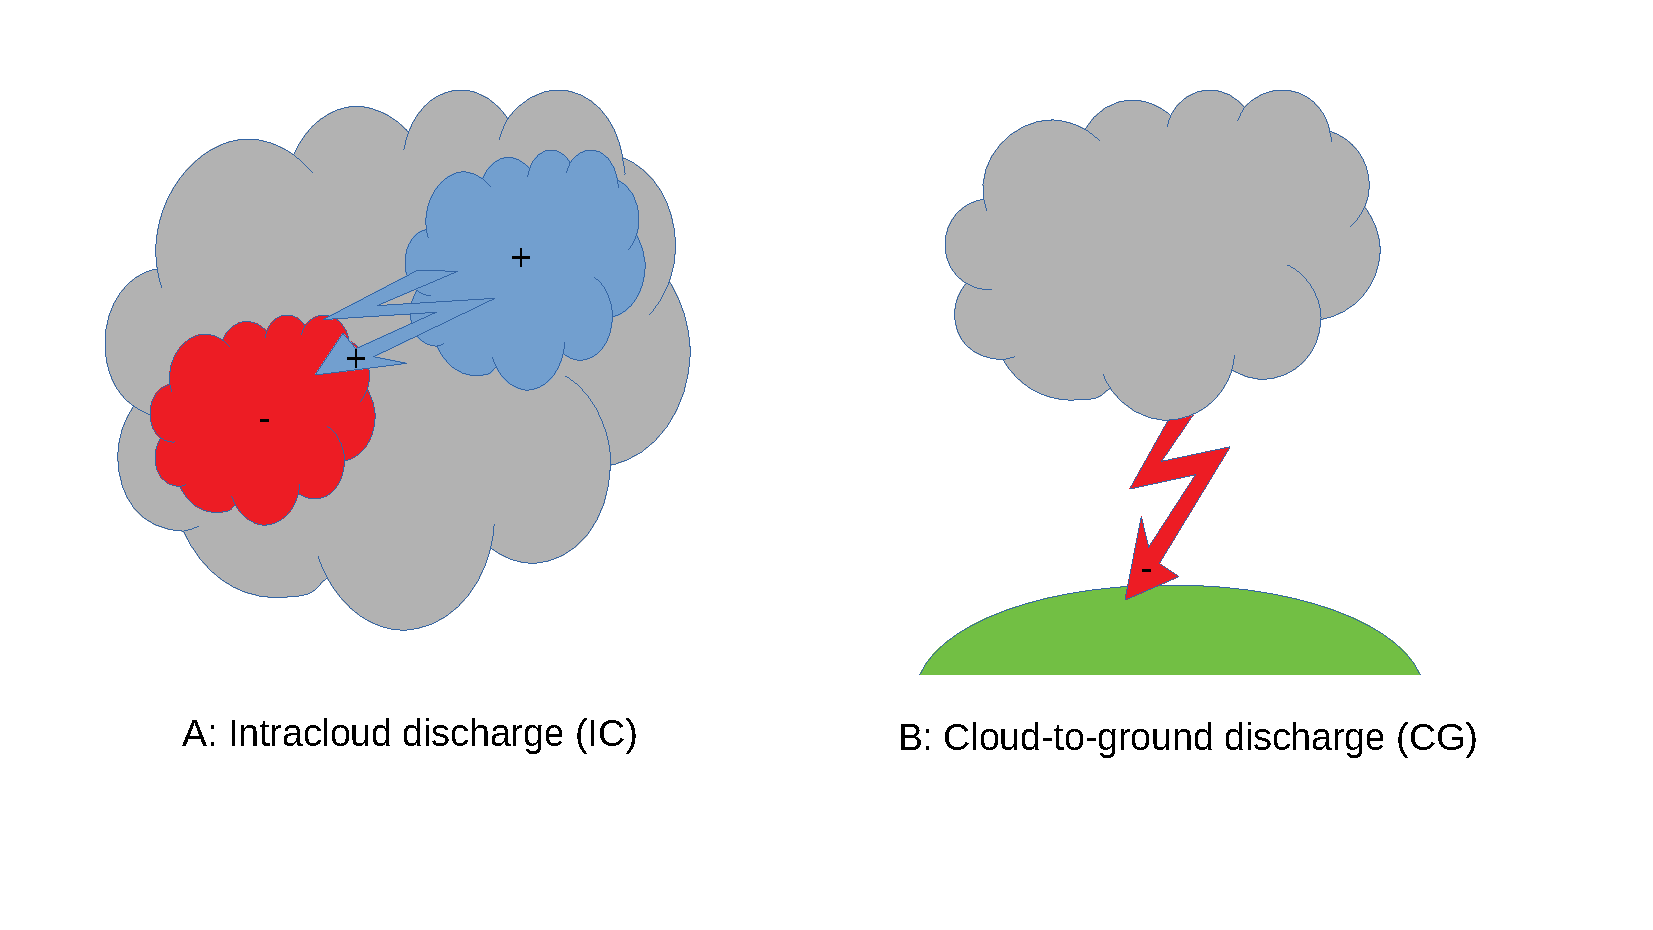
\includegraphics[width=\textwidth]{Figures/lyntyper.pdf}
    \caption{The two main categories of lightning. A shows an \acrfull{ic}, this could be between different storm cells or between different charge areas of the same storm cell. B shows a \acrfull{cg}, the polarity is defined by the charge change of earth. Negative cloud-to-ground (-CG) is defined by increase of negative charge at ground, and so positive cloud-to-ground (+CG) is defined by decrease of negative charge (increase in positive) at ground}
    \label{fig:lyntyper}
\end{figure}


\subsection{Winter lightning}
A phenomenon has been described in the Japanese meteorological field, where cold air from Siberia moves over the warm Tsushima current on the west coast of Japan. This leads to a strong temperature gradient between the cold air and the warm ocean, which causes convection. The  humidity supplied by the seawater leads to formation of hydrometeors. The resulting convection has been shown to produce lightning strikes and thunderstorms during winter (e.g. \cite{goto},\cite{michimoto2007}).

A similar phenomenon is observed of the west coast of Norway (e.g \cite{koeltzow2018}, \cite{montanya2016}). Cold air is brought from the arctic to the west coast of Norway where the ocean is warmed by the North Atlantic Current.The resulting temperature gradient may give rise to a convection and subsequent electrification.
 %This updraft and the creation of hydrometeors leads to an electrification that results in the aforementioned thunderstorms. 
 
\section{Helicopter Triggered Lightning}
An \acrshort{htl} is believed to be a phenomenon caused by the helicopter entering or coming close to an electrically charged part of a convective system. This can be attributed to the helicopter having a charge build-up during flight and then meeting a charge of opposite polarity. Alternatively the helicopter could induce a \acrshort{cg} by acting as part of the leader, see figure \ref{fig:triggertyper}. These different mechanisms are then analogous to \acrshort{ic} and \acrshort{cg} respectively. 

A positively charged discharge is believed to cause more damage to helicopters. The discharges to helicopters are also more often positive  (\cite{hardwick}).
%Helicopter triggered lightning is unique in that it does not occur during summertime, but only during the winter months (\cite{lande},\cite{wilkinson}).

\begin{figure}
    \centering
    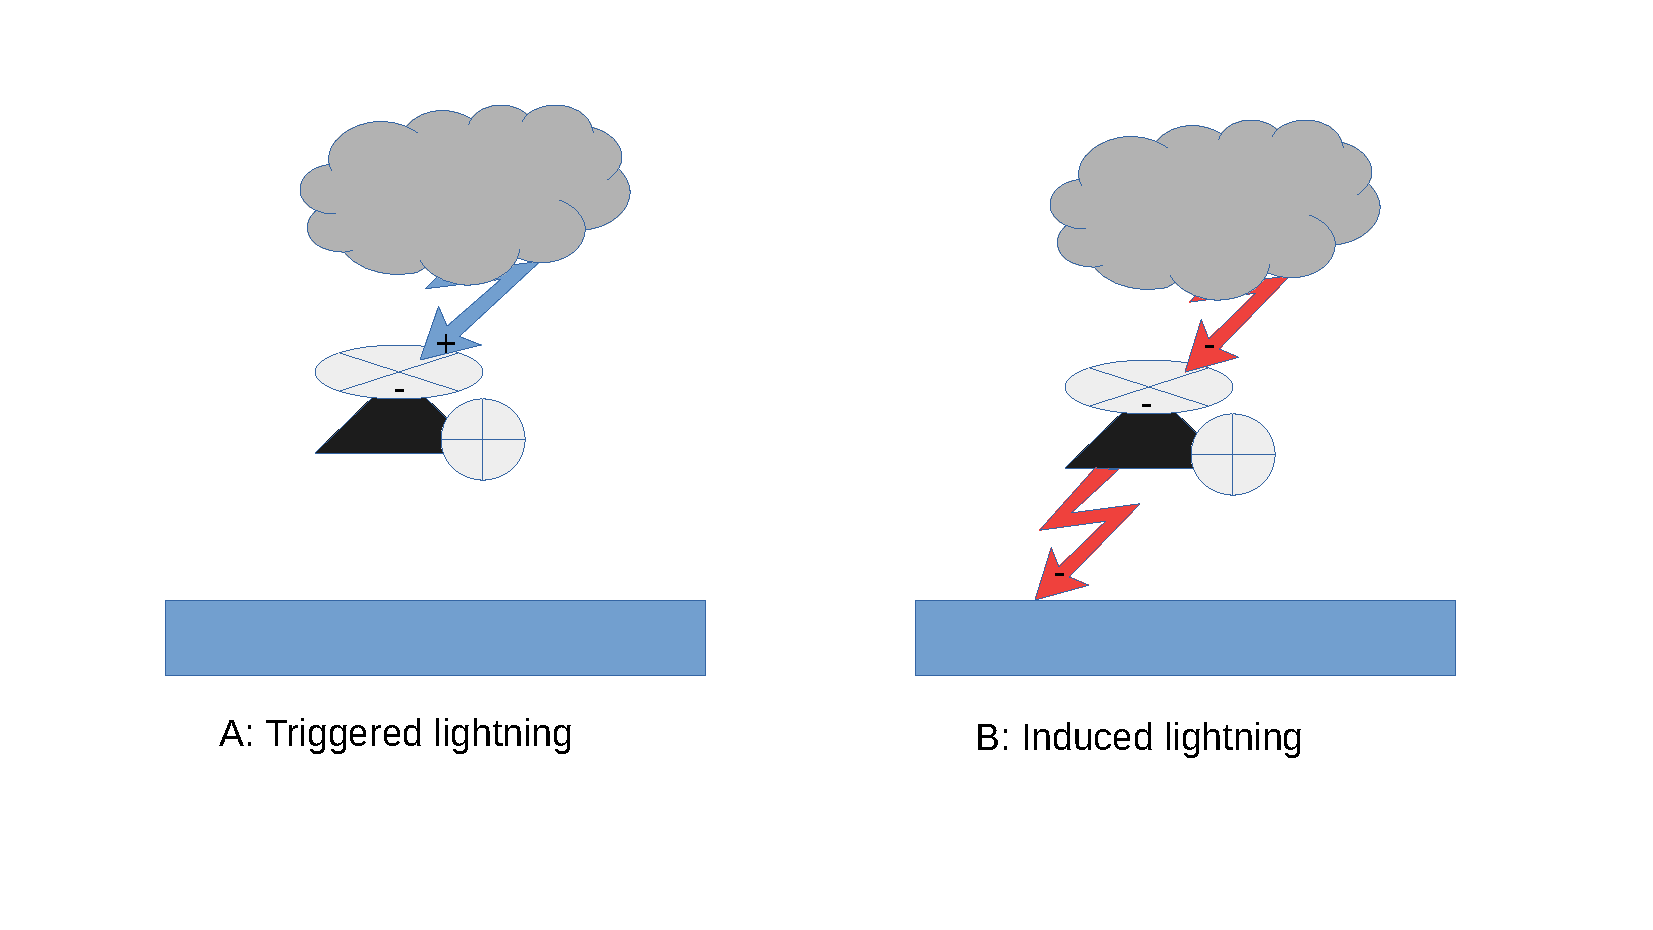
\includegraphics[width=\textwidth]{Figures/triggertyper.pdf}
    \caption{Illustration of different models for aircraft triggering. A shows the normal trigger situation, where the electrical discharge is grounded into the oppositely charged aircraft. B shows the situation where the aircraft is only acting as a pathway to the ground (Here ocean or land)}
    \label{fig:triggertyper}
\end{figure}

\subsection{Fixed Wing Triggered Lightning}

\acrfull{fwtl}, unlike \acrshort{htl}, is of less danger to both personnel and materials. Fixed-wing aircraft are generally hit in the main body. Fuel and vital electronics are also more protected in fixed-wing aircraft (\cite{Petrov12}). Helicopters are mainly hit through the rotor into the main body (\cite{lande}). 


\subsection{Forecasting HTL}
(\cite{lande}) looked at the common atmospheric conditions present for a \acrshort{htl}:
\begin{itemize}
 \item \acrfull{oat} at flight level near freezing point 
 \item frozen precipitation, as snow,ice and graupel.
 \item inside of or directly below clouds.
 \item within 5 nautical miles of a Cumulonimbus cloud.
\end{itemize}
This corresponds to convective activity, and especially zones of high electrification (Electrification is highest in the $0 - -10^{\circ}C$ temperature range. So what we want to find is local convective areas over oceans.



